\chapter{Lecture 7}
\chapterauthor{Kommireddy Bhargav Srinivas}
    
    \section{Languages in general}
    
    For any language in general we want to define the following.
    \begin{enumerate}
        \item Define the syntax, which consists of:
            \begin{enumerate}
                \item Abstract syntax (eg: AST)
                \item Concrete Syntax
                \item A Parser, which is a map from concrete syntax to abstract syntax.
                $$
                Parser : Concrete Syntax \rightarrow Abstract Syntax
                $$
            \end{enumerate}
        \item Define the Semantics, which consists of:
            \begin{enumerate}
                \item Semantic domains
                \item An evaluator, which is a map from abstract syntax to the domain of answers.
                $$
                Evaluator : Abstract Syntax \rightarrow Answers 
                $$
            \end{enumerate}
    \end{enumerate}
    
    \begin{figure}[htbp]
        \center
        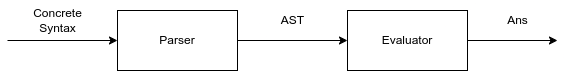
\includegraphics[scale=0.6]{images/lecture7/parser-evaluator.png}
        \caption{Parser Evaluator flow}
    \end{figure}
    
    \subsection{Language 0: ARITHMETIC}
    
    This is a simple language, which works on the integer domain and has the addition, subtraction and multiplication operators defined.
    
    The syntax of the expressions in this language can be defined as follows:
    
    
    \begin{align}
    expr & ::= Num&\\
         & \quad |\quad expr + expr&\\
         & \quad |\quad expr * expr&\\
         & \quad |\quad expr - expr
    \end{align}
    
    where Num represents any Integer.
    Any expression that matches this pattern is a syntactically valid expression in this language.
    
    The semantics of Arithmetic were covered in previous lectures.
    It will consist of the evaluation semantics (eval-ast : AST to Answer)

    The following is the racket implementation of the eval-ast function.
    \lstinputlisting[breaklines]{codes/evalast.rkt}

    \section{Language 1: IF+DIV}

    This language is syntactically a super set of ARITHMETIC. We introduce the if-then-else operator and also division. Division introduces new problems like dividing by zero. We also need to enforce that the condition given to if operator is a boolean.

    These situations cannot be predicted before the program is run for every program. They need to be caught during run-time. In these situations we would like to raise (or throw) errors (or exceptions).

    Now, the result of an expression is not just a number, it could be be a number or an error. There are two ways of dealing with errors, either they are treated specially and the whole execution of the program stops (In racket, you can achieve this using "invoke") and gives the error as the answer to the program. The other way is the treat errors as values, which are returned by the expression that produced the error.

    Errors like non-boolean if-condition (test) or incorrect type being provided to operators (eg: +, -) are called Type Errors
    
    The syntax of the expressions in this language can be defined as follows:
    
    
    \begin{align}
    e & ::= Num&\\
         & \quad |\quad e \quad + \quad e&\\
         & \quad |\quad e \quad * \quad e&\\
         & \quad |\quad e \quad - \quad e&\\
         & \quad |\quad e \quad / \quad e&\\
         & \quad |\quad if \quad e_{test} \quad e_{then} \quad e_{else}
    \end{align}

    The evaluation semantics have an extra rule for division (DIV) similar to addition and multiplication in ARITHMETIC. Along with that we need to define rules to evaluate if-then-else

    $$$$
    $$$$
    
    \begin{displaymath}
             e_{test} \implies \#t, \quad e_{then} \implies v \\
    \end{displaymath}
    % \begin{displaymath}
    \quad\quad\quad\quad\quad\quad\quad
    \textemdash\textemdash\textemdash\textemdash\textemdash\textemdash\textemdash\textemdash\textemdash\textemdash\textemdash\textemdash\textemdash\textemdash\textemdash\textemdash\textemdash\textemdash\textemdash\textemdash IF-TRUE
    % \end{displaymath}

    \begin{displaymath}
        if \quad e_{test} \quad e_{then} \quad e_{else} \implies v
    \end{displaymath}

    $$$$
    \begin{displaymath}
             e_{test} \implies \#f, \quad e_{else} \implies v \\
    \end{displaymath}
    % \begin{displaymath}
    \quad\quad\quad\quad\quad\quad\quad
    \textemdash\textemdash\textemdash\textemdash\textemdash\textemdash\textemdash\textemdash\textemdash\textemdash\textemdash\textemdash\textemdash\textemdash\textemdash\textemdash\textemdash\textemdash\textemdash\textemdash IF-FALSE
    % \end{displaymath}

    \begin{displaymath}
        if \quad e_{test} \quad e_{then} \quad e_{else} \implies v
    \end{displaymath}

    \section{Language-2: GLOBAL}

    A language doesn't need variables (eg: iptables) but programmers do. To make use of variables we need to introduce new constructs called identifiers and environment. Identifiers act as a proxy to values and the environment defines what value a specific identifier takes. (Read later: Combinatory Theory).

    The values that identifiers can take are called denotable values. The values that expressions can take are called expressible values. For the current language both are the same, but languages like C have them different (One cannot store a function in a variable in C).

    The syntax looks almost the same, except the fact that identifiers by themselves are also expressions.

    An environment is a map from identifiers to denotable values.
    
    $$Env: Identifiers \rightarrow Denotable values$$

    In this language, the denotable values is a disjoint union of Numbers and Booleans.

    $$ Denotable values \in Num + Bool $$

    The evaluation semantics change to include the environment as well. 

    \begin{figure}[htbp]
        \center
        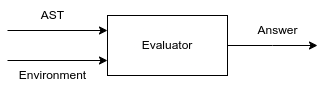
\includegraphics[scale=0.6]{images/lecture7/gloabal-eval.png}
        \caption{Global lang evaluator flow}
    \end{figure}

    When there is a mapping of an identifier in the environment, the identifier is said to be bound to that value. Introduction of identifiers creates a new type of error - Unbound identifier error. This happens when an identifier is used, but it is not bound to any value (It is a free variable.).

    While evaluating the AST if an identifier is encountered, a simple look up is performed in the environment and the corresponding value is taken. The identifier could be bound to an expression. In that case, the expression is evaluated and the corresponding value returned is substituted for the identifier.

    \textbf{Example}
    Expression is ( + x ( * y 2)) and the environment is 
    $$\Gamma = \{ x \mapsto 5, y \mapsto 3, z \mapsto 4\}$$

    We annotate the AST from bottom up get the final value. So we would first annotate x to 5, then y to 3, then get the result of multiplication as 6 and then the result of addition to be 11.

    \begin{figure}[htbp]
        \center
        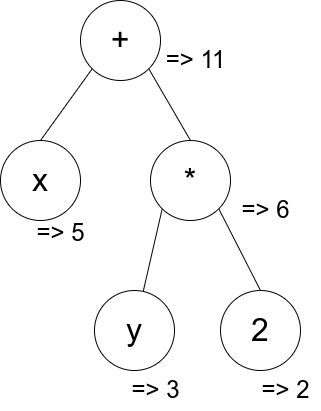
\includegraphics[scale=0.6]{images/lecture7/global_ex_ast.png}
        \caption{Global lang evaluator flow}
    \end{figure}
